\renewcommand*{\arraystretch}{1.5}
\noindent\begin{tabularx}{17cm}{|p{1.95cm}|X|}
	\hline
	number      & 13                                                          \\ \hline
	title       & Popular Tags per month in a country                                                           \\ \hline
	\multicolumn{2}{|c|}{ 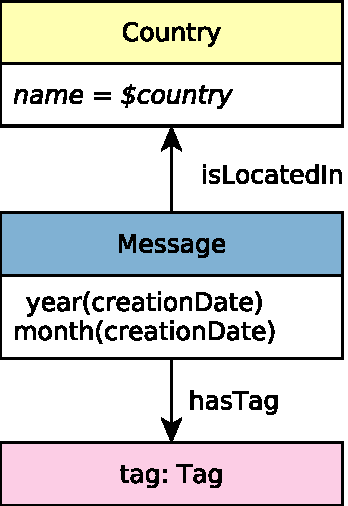
\includegraphics[scale=\patternscale,margin=0cm .2cm]{patterns/q13}} \\ \hline
	description & Find all Messages in a given Country, as well as their Tags.

For each group, find the 5 most popular Tags, where popularity is the
number of Messages (from within the same group) where the Tag appears.
 \\ \hline
	
	group by       &
	\multicolumn{1}{>{\raggedright}X|}{
		\varname{year}, 
		\varname{month}
		}\\ \hline
	
	parameters  &
	\renewcommand*{\arraystretch}{1.0}
	\vspace{-1.8ex}{\begin{tabularx}{14.2cm}{|c|l|p{2cm}|Y|} \hline
	\cellcolor{black!70} \color{white} $\mathsf{1}$ & \varname{country} & \cellcolor{gray!20} \vartype{String} & \\ 
	\end{tabularx}} \\ \hline
	result      &
	\renewcommand*{\arraystretch}{1.0}
	\vspace{-1.8ex}{\begin{tabularx}{14.2cm}{|c|l|p{2cm}|Y|} \hline
	\cellcolor{black!70} \color{white} $\mathsf{1}$ & \varname{year} & \cellcolor{gray!20} \vartype{32bitInteger} &year(message.creationDate) \\ \hline
	\cellcolor{black!70} \color{white} $\mathsf{2}$ & \varname{month} & \cellcolor{gray!20} \vartype{32bitInteger} &month(message.creationDate) \\ \hline
	\cellcolor{black!70} \color{white} $\mathsf{3}$ & \varname{popularTags} & \cellcolor{gray!20} \vartype{TagPairs} &(tag.name - String, popularity - 32bitInteger), sorted descending by popularity, then ascending by tag name \\ 
	\end{tabularx}} \\ \hline
	sort        &
	\renewcommand*{\arraystretch}{1.0}
	\vspace{-1.8ex}{\begin{tabular}{|c|l|c|} \hline
	\cellcolor{black!70} \color{white} $\mathsf{1}$ & \varname{year} & \cellcolor{gray!20} $\desc$ \\ \hline
	\cellcolor{black!70} \color{white} $\mathsf{2}$ & \varname{month} & \cellcolor{gray!20} $\asc$ \\ 
	\end{tabular}} \\ \hline
	limit       & 100                                                           \\ \hline
	choke points        &
	\multicolumn{1}{>{\raggedright}X|}{
		\chokepoint{1.2}, 
		\chokepoint{2.2}, 
		\chokepoint{2.3}, 
		\chokepoint{3.2}, 
		\chokepoint{6.1}
		}\\ \hline
\end{tabularx}
\clearpage